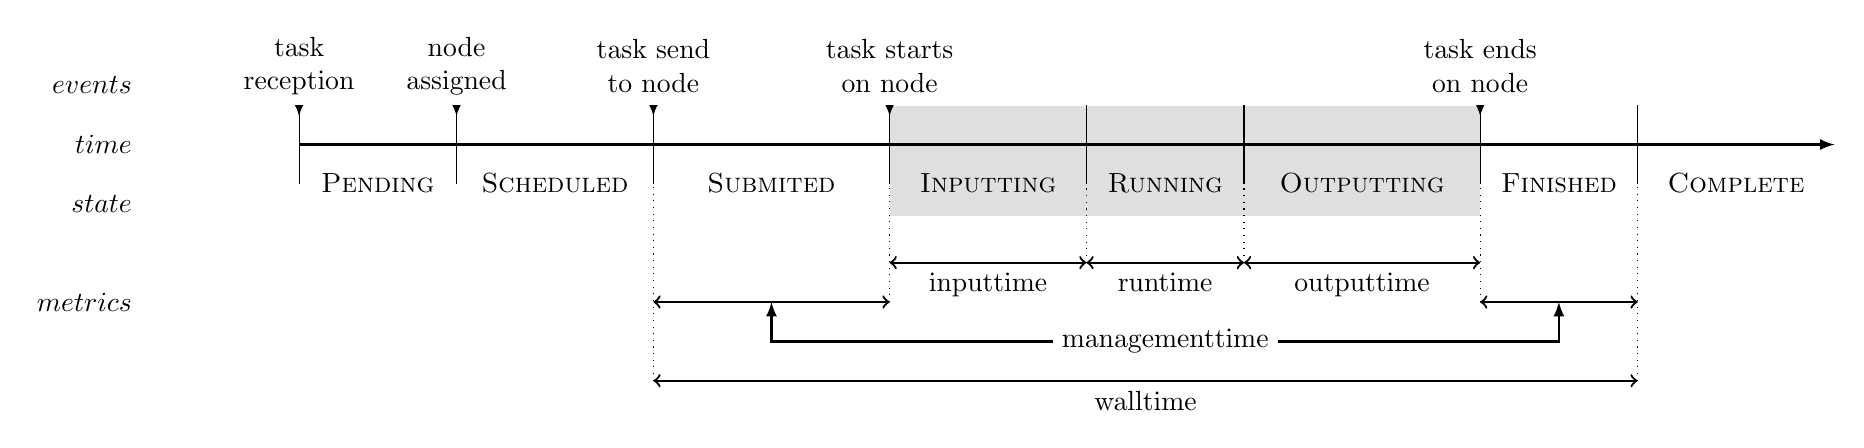
\begin{tikzpicture}[
legend/.style={anchor=east,align=right},
event/.style={align=center,outer sep=1},
status/.style={anchor=north,align=center,font=\sc},
metric/.style={<->,thick},
]
%legend
\node[legend]at(-1,0.75){$events$};
\node[legend]at(-1,0){$time$};
\node[legend]at(-1,-0.75){$state$};
\node[legend]at(-1,-2){$metrics$};

\node[rectangle,fill=gray!25,anchor=north west,minimum height=40,minimum width=213]at(8.5,0.5){};
%axis
\draw[-{latex},thick](1,0)--(20.5,0);
%marker - event - following status

%submition
\draw[{latex reversed}-](1,0.5)->(1,-0.5);
\node[event]at(1,1){task\\reception};
\node[status]at(2,-0.25){Pending};
%scheduling
\draw[{latex reversed}-](3,0.5)--(3,-0.5);
\node[event]at(3,1){node\\assigned};
\node[status]at(4.25,-0.25){Scheduled};
%sending
\draw[{latex reversed}-](5.5,0.5)--(5.5,-0.5);
\node[event]at(5.5,1){task send\\to node};
\node[status]at(7,-0.25){Submited};

%download
\draw[{latex reversed}-](8.5,0.5)--(8.5,-0.5);
\node[event]at(8.5,1){task starts\\on node};
\node[status]at(9.75,-0.25){Inputting};
%exec
\draw(11,0.5)--(11,-0.5);
\node[status]at(12,-0.25){Running};
%output
\draw(13,0.5)--(13,-0.5);
\node[status]at(14.5,-0.25){Outputting};
%finish
\draw[{latex reversed}-](16,0.5)--(16,-0.5);
\node[event]at(16,1){task ends\\on node};
\node[status]at(17,-0.25){Finished};
%complete
\draw(18,0.5)--(18,-0.5);
\node[event]at(18,1){};
\node[status]at(19.25,-0.25){Complete};

%metrics
\draw[dotted](5.5,-3)--(5.5,-0.5);
\draw[dotted](18,-3)--(18,-0.5);
\draw[metric](5.5,-3)--(18,-3)node[midway,below]{walltime};

\draw[dotted](8.5,-2)--(8.5,-0.5);
\draw[dotted](11,-1.5)--(11,-0.5);
\draw[dotted](13,-1.5)--(13,-0.5);
\draw[dotted](16,-2)--(16,-0.5);
\draw[metric](8.5,-1.5)--(11,-1.5)node[midway,below]{inputtime};
\draw[metric](11,-1.5)--(13,-1.5)node[midway,below]{runtime};
\draw[metric](13,-1.5)--(16,-1.5)node[midway,below]{outputtime};

\draw[metric](5.5,-2)--(8.5,-2);
\draw[metric](16,-2)--(18,-2);
\draw[{latex}-{latex},thick](7,-2)--(7,-2.5)--(17,-2.5)node[midway,fill=white]{managementtime}--(17,-2);

\end{tikzpicture}